% Activate the following line by filling in the right side. If for example the name of the root file is Main.tex, write
% "...root = Main.tex" if the chapter file is in the same directory, and "...root = ../Main.tex" if the chapter is in a subdirectory.
 
%!TEX root =  ../Thesis.tex

\chapter[Background Estimation]{Background Estimation}

Once the background has been reduced as much as practical using the trigger and kinematic cuts,
a reliable estimate of the shape and size of the remaining background is critical to optimizing
the exclusion limits.  In particular, since the reconstructed mass peak of the $b$-jets is so
broad in signal, a mis-estimation of the background shape can lead to systematic errors that
could wash out any possible signal (or worse, be mistaken for a signal where there is none).  

At the same time, the backgrounds in this analysis are challenging to estimate, either in Monte
Carlo or using data-driven methods.  Therefore, much of the work of this analysis is dedicated
to validating the background estimation and providing uncertainties for especially the shape 
of the background.  

\section{Background Estimation Strategy}
\label{sec:background_strategy}
As QCD is the dominant background in this analysis, it is important to understand
what flavors of QCD jets comprise the population of events that survive the cut
chain.  In order to do this, we apply the trigger and all cuts up to (but not including)
requiring a third $b$-tagged jet in the event; at this level of selection, we say
we are in the $bbx$ sample (because there are 2 $b$-tags already applied but the third
jet in the event can have any $b$-tag value.   

 The signal and background are then split into 3 exclusive regions, defined as follows:
\begin{itemize}
    \item bbb: one or more jets (in addition to the two triple-tagged jets) passing a tight (60\% working point)
 MV1 cut–-in effect, the full signal selection criteria
    \item bbloose: events failing the bbb classification but which have one or more jets passing a loose (80\%
 working point) MV1 cut
    \item bbanti: events that have no jets passing an 80\% MV1 cut-–effectively a veto on the presence of any
 b-tagged jets other than those firing the trigger
\end{itemize}


The bbanti and bbloose regions are depleted in signal and enriched in background, which allows
them to serve as control regions for the bbb signal region.  

Several background estimation strategies were attempted; we document all of those attempts 
in this section, including those that were not used in the final analysis.  The final strategy
uses the mass sidebands in the bbb signal region to estimate the background shape and
normalization in the signal region.  


\section{Background Estimation Method Based on Polynomial Background Model and Sideband Fitting}
The background consists almost exclusively of QCD with 2 or more real $b$-jets, which 
fortunately has a $m_{bb}$ spectrum that does not have any peaks or other difficult
structure above about 350 GeV.  Below that mass, the trigger turn-on curve becomes
a major feature of the spectrum, making it difficult to fit.  Above that mass, there
is a smoothly falling distribution that we fit with a Bernstein polynomial.

In a few words, this fit strategy proceeds in the following way:
\begin{itemize}
    \item Start with a mass point
    \item Using the signal MC as a guide, select a window in $m_{bb}$ that encloses the
signal peak, along with as much of the mass sideband (on either side) as possible
    \item Fit the Bernstein polynomial within that window, in each of the 
tag regions (bbb, bbloose, bbanti) as well as keeping the 3, 4, and 5+ jet bins separate
    \item Use the fit result for the background long with signal templates taken from
 MC to extract the 
cross section that can be excluded at a 95\% confidence level
    \item Repeat for the next mass point
\end{itemize}

Although we have signal MC with $m_A$ values as low as 250 GeV, this fit strategy only
begins to work above 350 GeV, because of the trigger turn-on curve.  

\subsection{Mass Windows}
A critical aspect of this strategy is selecting a mass window; large windows make for bigger
sidebands which can help the fit result (more information for it to use in making a prediction)
but also sometimes lead to convergence problems, since a larger window leaves more room
for the background to fluctuate, or have shape subtleties that the polynomial has difficulty
describing.  In fact, an early iteration of this fit strategy used the same large $m_{bb}$ 
window \[320, 900 GeV\] but the background shape over that large region changes enough that
the error matrix of the fit result was not positive-definite, leading to uncertainties that 
could not be quantified reliably.   

The final choices of mass windows are documented in Table~\ref{tab:mass_windows}.

%--------------------------------------------------------
\begin{table}
   \caption{The mass window used when fitting each signal mass point. \label{tab:mass_windows} }
    \begin{tabular}{ c c c }
    mass (GeV) & lower edge & upper edge \\
    250        & 1.68682  & \\
    280        & 1.92318 & \\
    310        & 2.50849 & \\
    350        & 3.23507 & \\
    400        & 3.93561 & \\
    450        & 4.71906 & \\
    500        & 5.59454 & \\
    550        & 6.84368 & \\
    600        & 8.11044 & \\
    650        & 9.26688 & \\
    700        & 10.3760 & \\
    800        & 12.5049 & \\
    \end{tabular}
\end{table}

%--------------------------------------------------------








\section{Attempted (But Not Used) Background Estimation Methods}
 
A control-region-based binned background fit was attempted before the polynomial background fit was selected
for the final version of the analysis.  This strategy is documented here, for the
benefit of future analysts.  The strategy ultimately rests on having bb QCD MC for validation
of a key assumption (that the shape of the $m_{bb}$ distribution is the same in QCD 
regardless of the flavor of the third jet in the event).  The details of this sample
are documented in Section~\ref{sec:bb_qcd_mc}, but unfortunately it was not produced in
large statistics due to ATLAS-wide production problems.   

For the alternative fit method documented here , we use the bbanti (and bbloose) control regions to predict the background shape in the bbb signal region.
The background estimation strategy is to fit the $m_{bb}$ distribution in these three tag bins together. In
 practice, the bbanti bin dominates that fit because it has much higher statistics than the other two bins. In
 addition, we expect the bbanti bin to be heavily dominated by events that have exactly 2 b-jets, with the
 third jet being charm or light. Therefore, when we fit the three mbb distributions together, we are making
 an important assumption: the $m_{bb}$ distribution of the leading 2 jets is independent of the truth flavor of the third jet.

This assumption is validated in several ways, which are detailed in this section.
\begin{itemize}
    \item Simple tag-based data-driven shape check
    \item Matrix method data-driven shape check
    \item bb QCD MC shape check
\end{itemize}
 We also apply a jet-pT -based reweighting, to correct for any biases that might be introduced when
 b-tagging is applied to the third jet, which is also discussed in this section.


\subsection{Shape Check After Applying $b$-Tagging}
\subsection{Shape Check after Applying $b$-Tagging}
A simple first check of our background shape assumption is done on by plotting the mbb distribution
 in data for the bbb, bbloose and bbanti distributions tag bins; we would expect these to have different
 admixtures of bottom, charm and light jets in the third jet and so differences in these $m_{bb}$ distributions
 would hint at our assumption being violated. There are 12,308 bbb events, 9,049 bbloose, and 76,123
 bbanti events in 10\% of the 2012 data. The three mbb distributions are plotted in Figure~\ref{fig:mbb_data}, where the
 out-of-the-box distributions are shown on the left and the distributions are normalized to the same area
 on the right. No shape differences are apparent. Figure~\ref{fig:mbb_data} shows the distributions normalized to the
 same area and with a logarithmic y scale for easy shape comparison; no major shape differences appear
 there either.

\begin{figure}[hbt]
  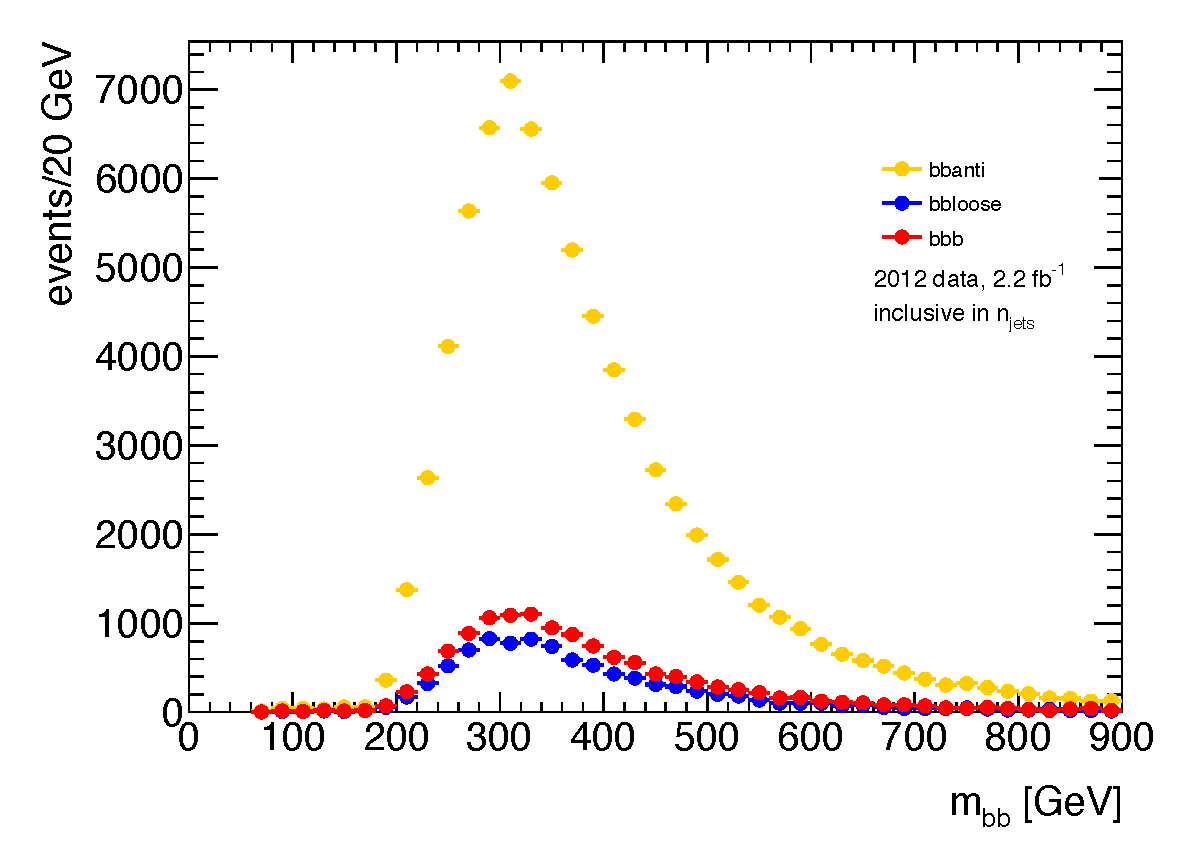
\includegraphics[width=0.5\linewidth]{BackgroundEstimation/images/mbb_bbb_bbloose_bbanti_r200-215.pdf}
  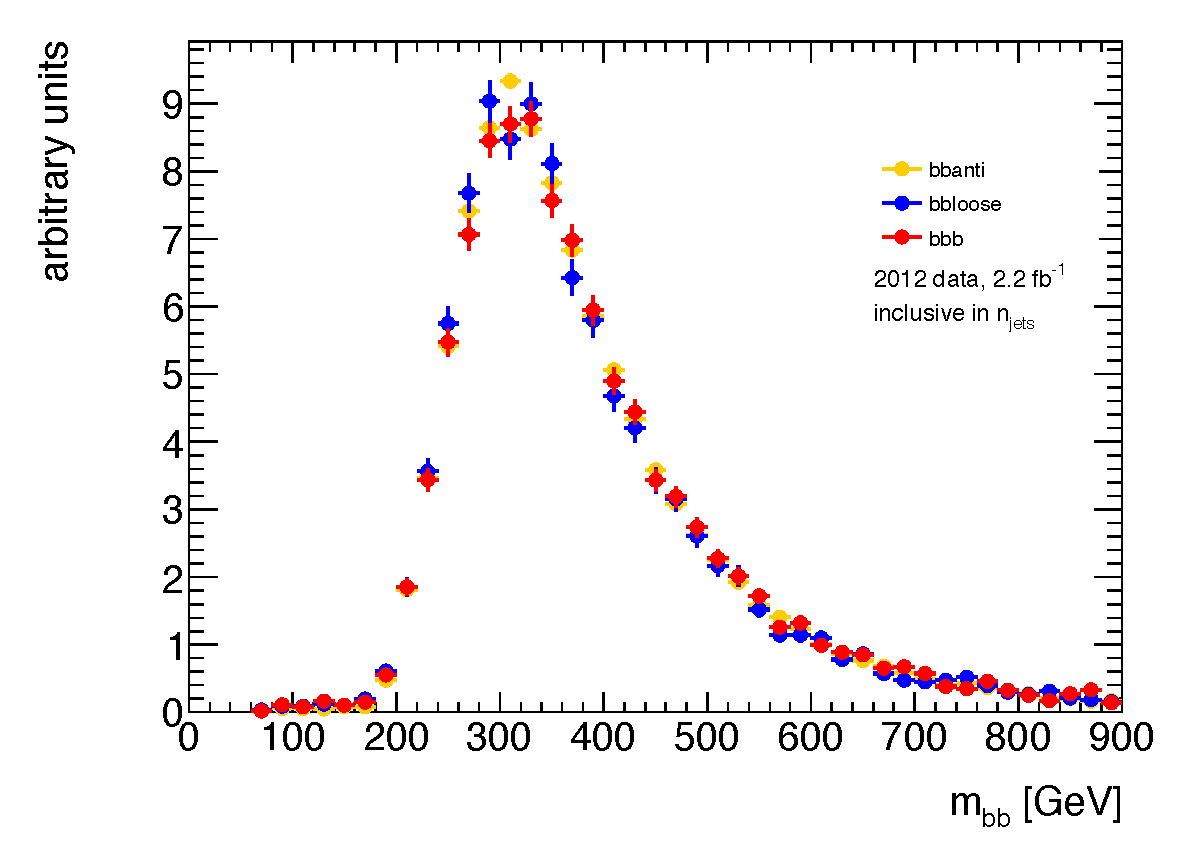
\includegraphics[width=0.5\linewidth]{BackgroundEstimation/images/mbb_bbb_bbloose_bbanti_r200-215_normalized.pdf}
%  \label{fig:mbb_data}
  \caption{$m_{bb}$ distributions in data, based on the $b$-tag status of the third jet. 
    \label{fig:mbb_data} }
\end{figure}


\subsection{Shape Check Using the Matrix Method}








\subsection{The Matrix Method}
The matrix method is a data-driven way to use the tag distributions of the data (which can be accessed experimentally) to compute the flavor distributions (which cannot be directly found experimentally).  After the matrix method has been applied, the result are $m_{bb}$ distributions that are broken apart based on the predicted truth flavor (bottom, charm, or light) of the third jet.  Hypothetically,
the matrix method can be used to do a completely data-driven prediction of the $m_{bb}$ distribution
for each possible truth flavor of the third jet.  In practice, we find that the errors on the matrix
method prediction are too large to use it as the primary background estimation strategy, or to validate
the assumption that the $m_{bb}$ distribution is independent of the flavor of the third jet.  

Recall that after the trigger and all cuts (including $b$-tagging on the third jet) the QCD background will be of two major types:

\begin{itemize}
    \item a reducible portion where one or more light or charm jets get mistagged as $b$-jets
    \item an irreducible portion in which there are three or more true $b$-jets from the
hard scatter and/or gluon splitting
\end{itemize}


The goal of the matrix method is to disentangle these backgrounds, and allow us to describe the shape of the $m_{bb}$ distribution from $bbb$ events
in a data-driven way.  In what follows, we adopt the convention where lowercase letters indicate flavors
that are ``known,'' either via assumption or via truth-matching using MC.  Thus $bbb$ refers to an event where the true flavor of the three jets is bottom.  Uppercase letters,
on the other hand, denote a presumed flavor, most likely because either a jet has been $b$-tagged or reweighted by the matrix method.  An event which has a third jet
that is $b$-tagged (but could still be a mistagged light or charm jet) would be
denoted $bbB$.  

As part of the cut chain, two jets have been ``triple-tagged'' ($b$-tagged
at L2, EF and offline) and so, modulo a systematic which we estimate separately, 
those events are treated as being a 100\% pure sample of events with at least 2 real $b$-jets.
Then the issue becomes to diagnose the flavor of the third jet in the event,
which may or may not be a $b$-jet and may or may not be $b$-tagged.  Since
reliable QCD MC with at least 2 real $b$ quarks can be hard to generate, especially
in high statistics once the cut chain has been applied, a data-driven method for
estimating the flavor of the third jet provides the primary means of estimating
the background from mistagged light or charm QCD jets.  The matrix method allows
us to use a data-driven quantity, the MV1 distribution of the third jet
solve for the (experimentally inaccessible) distribution of truth flavor in data events.

\subsubsection{Mathematics of the Matrix Method}
There are three unknown quantities being sought when we apply the matrix method: the amount of $bbB$, $bbC$, and $bbL$ in our sample after all cuts except the b-tag on the third jet has been applied.   Since there are three unknowns, we must write a system of three linear equations, and we must have three tag categories, which appear on the left hand side of equation \ref{eq:matrix1}.  There are three tag categories:
	
	\begin{itemize}
		\item $N_{tight}$: third jet has an MV1 value that is at least as high as the 60\% efficiency working point (the same as the bbb category introduced in Section~\ref{sec:background_strategy})
		\item $N_{loose}$: third jet has MV1 value that is at or above the 80\% efficiency working point, but below the 60\% efficiency working point (same as bbloose)
		\item $N_{anti}$: third jet has MV1 value below the 80\% working point (same as bbanti)
	\end{itemize}

All jets being examined will fall into exactly one of these categories.

        \begin{equation}
            \begin{bmatrix} \scriptstyle
            N_{tight} \\ \scriptstyle
            N_{loose} \\ \scriptstyle
            N_{total}
            \end{bmatrix}    
            = 
            \begin{bmatrix} \scriptstyle
                \epsilon^b_{tight} & \scriptstyle \epsilon^c_{tight} & \scriptstyle \epsilon^l_{tight} \\  \scriptstyle
                \epsilon^b_{loose} - \epsilon^b_{tight} & \scriptstyle \epsilon^c_{loose} - \epsilon^c_{tight} & \scriptstyle \epsilon^l_{loose} - \epsilon^l_{tight} \\      \scriptstyle
                1.0 - \epsilon^b_{loose} & \scriptstyle 1.0 - \epsilon^c_{loose} & \scriptstyle  1.0 - \epsilon^l_{loose}
            \end{bmatrix}
            \begin{bmatrix} \scriptstyle
                N^b \\ \scriptstyle
                N^c \\ \scriptstyle
                N^l
            \end{bmatrix}
        \label{eq:matrix1} 
        \end{equation} %\label{eq:matrix1}

Once the tag counts $N_{tight}$, $N_{loose}$ and $N_{anti}$ are found in data, the equation in \ref{eq:matrix1} can be inverted to solve for the flavor composition of the sample, as shown in \ref{eq:matrix2}.


        \begin{equation}
            \begin{bmatrix} \scriptstyle
                N^b \\ \scriptstyle
                N^c \\ \scriptstyle
                N^l
            \end{bmatrix} 
            = 
            \begin{bmatrix} \scriptstyle
                \epsilon^b_{tight} & \scriptstyle \epsilon^c_{tight} & \scriptstyle \epsilon^l_{tight} \\  \scriptstyle
                \epsilon^b_{loose} - \epsilon^b_{tight} & \scriptstyle \epsilon^c_{loose} - \epsilon^c_{tight} & \scriptstyle \epsilon^l_{loose} - \epsilon^l_{tight} \\      \scriptstyle
                1.0 - \epsilon^b_{loose} & \scriptstyle 1.0 - \epsilon^c_{loose} & \scriptstyle  1.0 - \epsilon^l_{loose}
            \end{bmatrix}
            ^{-1}
            \begin{bmatrix} \scriptstyle
            N_{tight} \\ \scriptstyle
            N_{loose} \\ \scriptstyle
            N_{total}
            \end{bmatrix}  
        \label{eq:matrix2} 
        \end{equation} %\label{eq:matrix2}

The b-tagging efficiencies that comprise the matrix are $p_T$ and $\eta$ dependent, so we create a 2D binning and create a different matrix and set of tag counts for each bin.  



\subsection{Matrix Method Validation and Errors}
\subsubsection{Validation Studies}
Two aspects of the matrix method result must be validated: the overall number of $B$, $C$ and light jets predicted (i.e. the normalization) and the shape of the $m_{bb}$ distribution when reweighted by the matrix method (i.e. that any shape differences in the $m_{bb}$ distributions based on the flavor of the third jet must propagate through in the matrix method predictions).  Toy MC provides a laboratory for performing these checks.  

First, we generate a Toy MC sample where the fraction of $b$, $c$, and light 
jets is known exactly, then these samples are sent through the analysis framework for $b$-tagging and 
then the counts in those $b$-tag categories used to predict the flavors of the original sample; 
the input and output flavor normalizations match to within a few percent (the difference results from statistical fluctuations, 
since the kinematic distributions of the Toy MC are allowed to have random fluctuatioons that can then propagate through to the final result).  
%----------------------------------------------
\begin{table}
\centering
\caption{Results of the matrix method normalization tests when run on a Toy MC sample of 
    900,000 total events.  The matrix method is run with the same efficiencies that
    are used to generate the toy MC samples, so the errors are statistical only.
    \label{tab:mm_toy_mc}   }
  \begin{tabular}{cccc}
     \hline \hline
     Flavor & Truth Events & MM Predicted Events & \% Difference  \\ \hline
     b   & 45,000 & 45,602 & +1.3\% \\
     c   & 90,000 & 86,938 & -3.4\% \\
     light & 765,000 & 767,458 & +0.3\% \\
     \hline     \end{tabular}
\end{table}
%----------------------------------------------

A second task for the Toy MC studies is to validate the $m_{bb}$ shapes.  Even if the normalization is perfect coming out of the matrix method, a major concern is the shape of the $m_{bb}$ distribution based on the truth flavor of the third jet.  The shape prediction is validated in Toy MC, by changing the shape of the $m_{bb}$ distribution based on the truth flavor of the third jet and checking to see if the shape differences propagate through.  



\subsubsection{Statistical and Systematic Errors}
\begin{itemize}
    \item Binning studies to quantify statistical errors that can result from having a fine \pt-$\eta$ binning in the $b$-tagging efficiencies
    \item Systematics associated with the $b$-tagging scale factors
\end{itemize}



\subsection{MC-Based Validation of Shape Assumption}


















%
%The background estimate is crucial to the analysis.  The QCD cross section at a hadron machine like the LHC is quite large; only a small subset of QCD events have 3 or more b-jets, but b-tagging does not have perfect performance and we expect a large contribution from QCD events in which one or more light or charm jets are b-tagged.
%
%The b-tagging in the trigger provides a handle for controlling the mistag background.  The L2, EF and offline MV1 b-tags are independent of each other, which is to say that (for example) the EF b-tagging decision on a given jet does not take into account whether the jet was tagged in L2, so we can improve the purity of our b-jet sample by requiring that the same jet pass L2, EF and MV1 tags.  


%  \begin{table}[hbt]
%
%    \begin{tabular}{l | l | c | c || c | c }
%    \multicolumn{2}{c}{}  & \multicolumn{2}{c}{Signal MC} & \multicolumn{2}{c}{Unbiased Data} \\
%      X         & Y         & sig-like & bkgd-like   &   sig-like & bkgd-like \\
%      \hline
%      EF        & L2        & 0.917    & 0.248 &   0.424       & 0.035 \\
%      \hline
%      L2        & MV1 (80)  & 0.675    & 0.031 &       0.510       & 0.077 \\
%      EF        & MV1 (80)  & 0.824    & 0.090 & 0.515       & 0.050\\
%      L2 and EF & MV1 (80)  & 0.676    & 0.036 & 0.414       & 0.031 \\
%      MV1 (80)  & L2 and EF & 0.977    & 0.434 & 0.640       & 0.076 \\
%      \hline
%      L2        & MV1 (70)  & 0.716    & 0.060 & 0.652       & 0.086\\
%      EF        & MV1 (70)  & 0.867    & 0.131 & 0.665       & 0.060 \\
%      L2 and EF & MV1 (70)  & 0.721    & 0.060 & 0.563       & 0.038\\
%      MV1 (70)  & L2 and EF & 0.954    & 0.340 & 0.538       & 0.034\\
%      \hline
%      L2        & MV1 (60)  & 0.757    & 0.101 & 0.762       & 0.095\\
%      EF        & MV1 (60)  & 0.903    & 0.193 & 0.779       & 0.070 \\
%      L2 and EF & MV1 (60)  & 0.765    & 0.103 & 0.692       & 0.045\\
%      MV1 (60)  & L2 and EF & 0.902    & 0.250 & 0.429       & 0.015\\
%    \end{tabular}
%    \\
%    \vspace{2mm}

%\caption{  The acceptance of a cut on variable X given that the events have
%  already passed (sig-like) or failed (bkgd-like) a cut on variable Y.}
%  \end{table}
  


%The third jet in the event, however, will not be tagged by the trigger.  The jet will be tagged offline, but even after the offline tagging we expect there will be many events in which the third jet is not a b-jet, but is a mistagged light or charm jet.  The exact size of this background for light jets is given by equation \ref{eq:mistag}, and a similar equation can be written for charm jets.

%  \begin{equation}
%	N_{mistagged\ light\ jets} = N_{light\ jets} \times \epsilon_{light\ jet\ passing\ tag}
%\end{equation} \label{eq:mistag}

%The light mistag efficiency $\epsilon_{light\ jet\ passing\ tag}$ is computed and calibrated by the b-tagging performance group (see the b-tagging chapter for further details), so we need to compute the composition of light or charm jets in the original sample in order to estimate their contamination after b-tagging has been applied.  

%The QCD background is notoriously difficult to model in MC, and we find unacceptably low statistics in MC after our analysis cuts have been applied, so we use the data-driven matrix method to compute the QCD background composition as accurately as possible.  The matrix method makes use of the known efficiencies for tagging b, c and light jets, as well as information about how many jets pass a given b-tag, to arrive at 



%\section{Matrix Method Strategy and Mathematics}





%\section{Matrix Method Binning} \label{sec:matrix_method_binning}
%The tag counts $N_{tight}$, $N_{loose}$ and $N_{anti}$ obey Poisson statistics, and are prone to statistical fluctuations that can propagate through the method and make the flavor predictions less accurate.  As the number of events in a given bin goes up, the relative Poisson error goes down and the method generally gives better performance.  However, having bins that cover a large region in $p_T$/$\eta$ phase space comes with the complication that the b-tagging efficiencies might vary within that phase space, so assigning a single efficiency value in that bin would wash out the variation and create larger systematic errors.

%The matrix method binning thus must optimize the tradeoff between small statistical errors (large bins) and small efficiency-related systematic errors (small bins).  In order to probe the statistical error on the bin as a function of bin statistics, figure \ref{fig:bin_stats_errors} shows the performance (defined as (prediction-truth)/truth for a given flavor) of the matrix method versus the bin statistics.  The bin statistics is defined as the total number of events in a given bin, so it encompasses all tag categories.

%The results seen in Figure \ref{fig:bin_stats_errors} allow us to make several insights.  At low bin statistics, where Poisson errors are expected to have the most impact, the performance shows the most variation, indicating larger relative errors.  As the bin statistics increase, the performance converges asymptotically on 0, indicating that, for example, there is no great change in statistical errors between 400 events and 1000 events per bin.  With this in mind, and estimating that 300 events per bin is approximately where this asymptotic behavior becomes dominant, the bins should be drawn such that they each contain at least approximately 300 events.

% this figure is made by executing "binning_study" in matrix_method_systematics.py
%   the drawing is done in plotPerformanceVsStats in mms_plots.py
%   and generally lives in h4b/python/dovers.eps
%\includegraphics[width=\textwidth]{/Users/caitlinmalone/Documents/Thesis/BackgroundEstimation/images/dovers.eps}
%\label{fig:bin_stats_errors}

%\section{Closure Tests}
%Closure tests are applications of the matrix method in a very controlled situation, where the expected prediction of the method is easy to predict.  Closure tests allow bugs in the method to be more readily seen, so they can be targeted for further study.  In this implementation of the matrix method, closure tests are performed by deriving the efficiencies from a sample which is then used as the input to the matrix method.  

%\begin{enumerate}
%	\item In a Monte Carlo QCD sample, count the number of jets of a given flavor
%	\item In the same sample, count the number of jets of a given flavor passing a b-tag cut of a given working point 
%	\item Divide (2) by (1) to derive the b-tagging efficiency for that flavor and working point in QCD MC
%	\item Repeat for all flavors and working points
%	\item Run matrix method with the QCD MC events as the inputs and the derived efficiencies as the matrix inputs
%\end{enumerate}

%Mathematically, since the flavor counts can be expressed in terms of the efficiencies and the tag counts, the equations of the matrix method should give perfect predictions of the flavor counts in the QCD MC sample, modulo rounding or matrix inversion errors.  

%The closure test method outlined above can be repeated bin-by-bin for testing closure of each bin individually.  Then the difference between the prediction and MC truth in each bin for each flavor can be plotted; the difference should be very close to zero.

%\section{Statistical Errors}



%\section{Systematic Errors}
%b-tagging systematics in VH:  https://cds.cern.ch/record/1551231/files/ATL-COM-PHYS-2013-697.pdf
%Unlike statistical errors, the systematic errors of the matrix method do not decrease as the method is run over more jets.  In practice, the systematic errors of the method arise from deviations between the efficiencies that are used in the matrix and the true efficiencies of the input sample.  Such deviations can come from several places, most notably sample dependence and Monte Carlo vs. data differences. 

%The sample on which the efficiencies are derived can affect what values are computed for the efficiencies themselves.  The b-tagging efficiencies at ATLAS are computed on a $t\bar{t}$ sample, which generally does not have identical kinematics to a QCD sample.   





\subsection{Non-QCD Backgrounds}
\label{sec:non_qcd_bkgs}

\subsubsection{All-Hadronic $t\bar{t}$ Background}
When $t\bar{t}$ decays all-hadronically, it can create events with several high-$p_T$
jets and 2 or more $b$-tagged jets (where the $b$-tags come from both real $b$-quarks
and from mistagged light flavor).  We anticipate that, because it has a production
cross section that is much smaller than QCD, $t\bar{t}$ will not be a major background.
We confirm this assumption in MC by using the all-hadronic $t\bar{t}$ sample summarized
in Table~\ref{tab:ttbar_params}.


We find that in MC, all-hadronic $t\bar{t}$ has an efficiency of 7.5\% after
the EF\_2j35\_loose\_j145\_j35\_a4tchad trigger, and approximately 2\% efficiency
in the offline cuts relative to the trigger.  Estimating the $t\bar{t}$ cross section
as 165 pb, and a 44\% branching ratio in the all-hadronic decay channel, this gives
a 0.11 pb $t\bar{t}$ cross section expected after the trigger and offline cuts.  In the
full 2012 dataset, this amounts to about 2400 events.  While
this is not a negligible cross section compared to the signal, it is more than an
order of magnitude smaller than the QCD background.

In addition to checking the magnitude of the $t\bar{t}$ background, we check the shape
for any shape differences in the $m_{bb}$ distribution depending on the tag status of the
third jet, and do not find any major discrepancies that point toward $t\bar{t}$ as a
potential peaking background in the signal region. The $m_{bb}$ distributions in the
bbb, bbloose and bbanti bins for the all-hadronic $t\bar{t}$ can be found in Figure
~\ref{fig:ttbar_mbb}.




\begin{figure}[hbt]
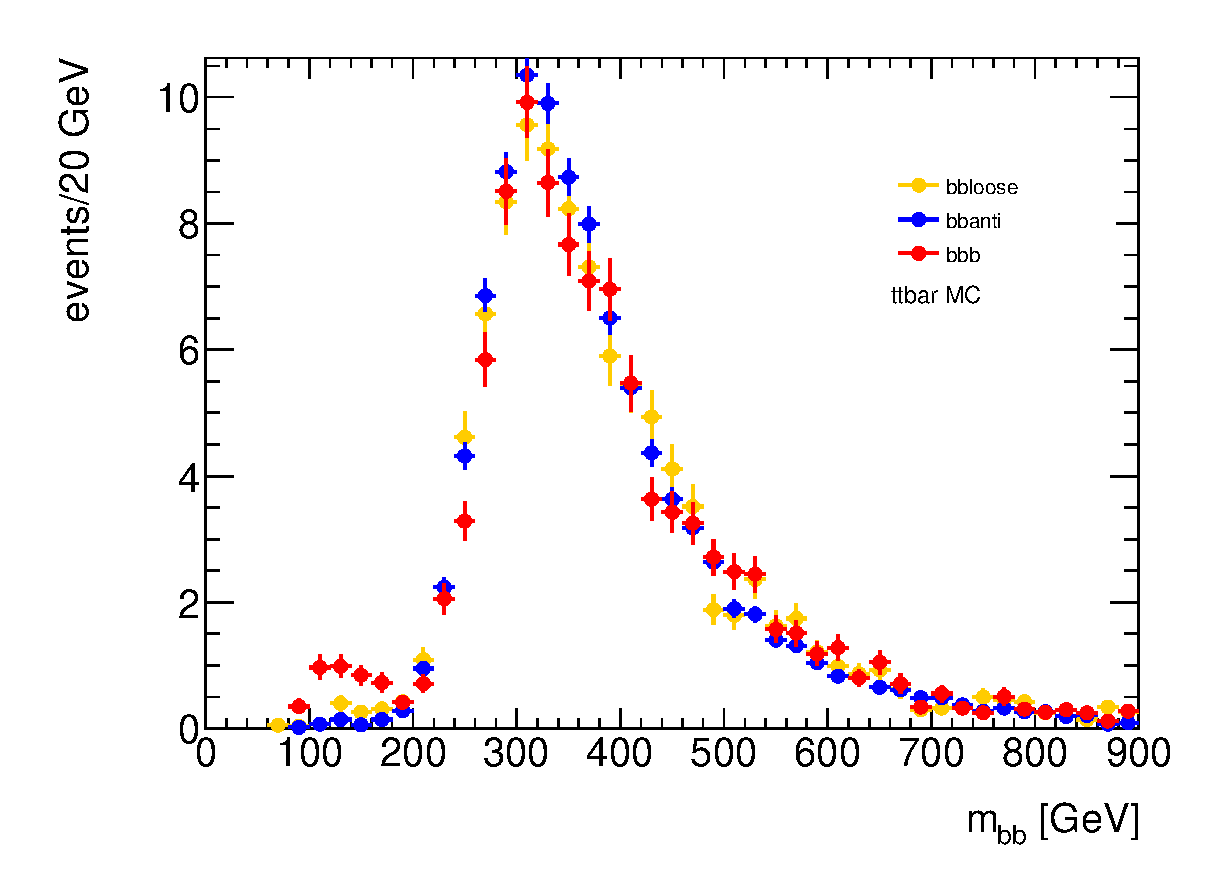
\includegraphics[width=0.45\linewidth]{BackgroundEstimation/images/mbb_compare_bbb_bbloose_bbanti_ttbar.eps}
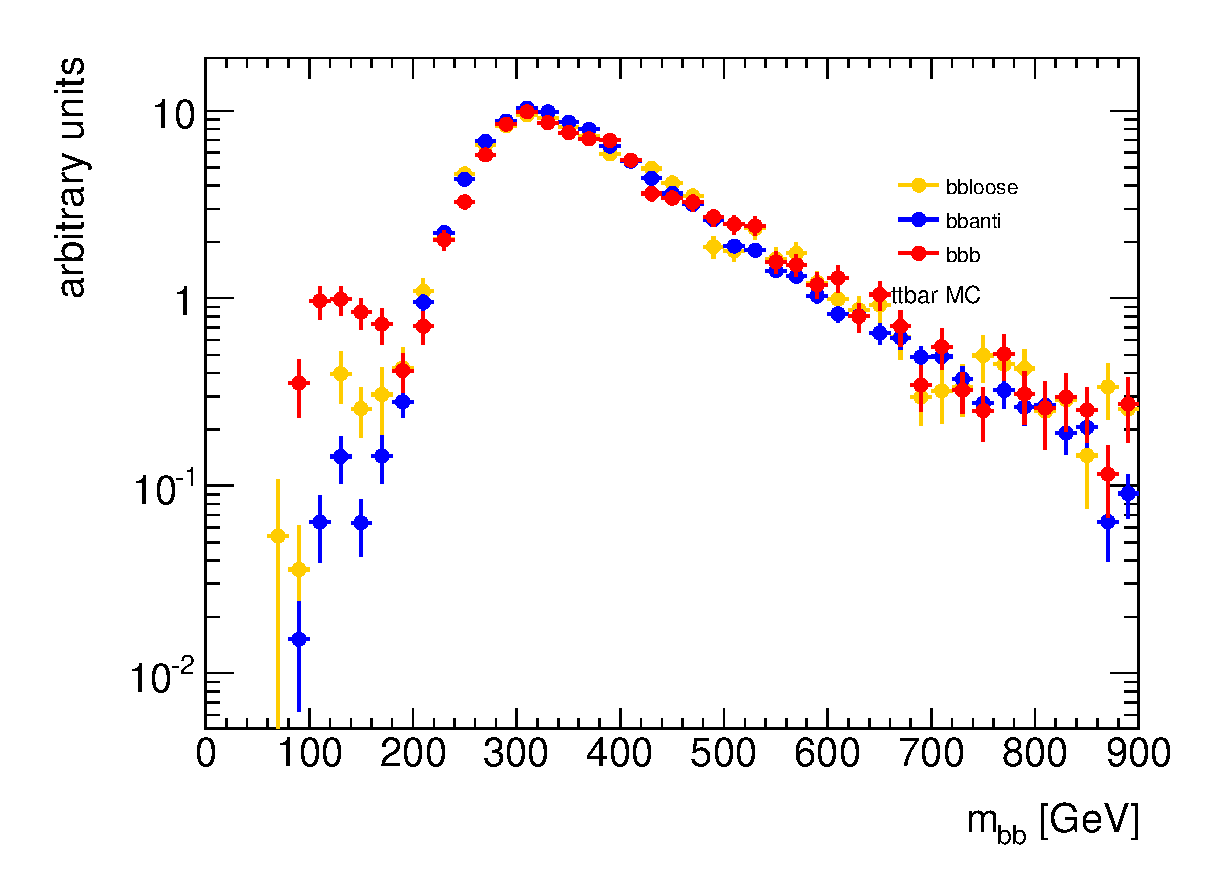
\includegraphics[width=0.45\linewidth]{BackgroundEstimation/images/mbb_compare_bbb_bbloose_bbanti_ttbar_logy.eps}
\caption{The $m_{bb}$ distributions for all-hadronic $t\bar{t}$ MC after the trigger and all offline cuts are applied (linear Y axis on the left, logarithmic scale on the right).  In addition to the overall cross-section, we also want to probe any shape differences that arise when the tag status changes on the third jet in the event.  No significant shape differences are seen.}
\label{fig:ttbar_mbb}
\end{figure}



              \subsubsection{Vector Boson + Jets Background}
